\chapter{Skill-biased technical change}

% Wage inequality rising since 1960s, especially in the top half of the earnings distribution. In the United States, where real wages for unskilled workers have declined, on average, since 1970, the skill premium for college graduates has grown significantly. But changing distribution of education doesn't explain the rise in inequality. Robust to industry (shown with census data.)

% Causes of SBTC include (a) cheaper capital/computers, (b) institutional changes. Skills can be considered (a) complement physical+computer capital, or (b) particular skills needed for rapid change. Other explanations incude international openness and trade, increasing competition for jobs at low end of spectrum. Further, labor institutions are changing, especially weaker unions.
                
%US, Canadian and British experience particularly pronounced. Europe experienced similar increase in inequality; borne out more in unemployment than wage (institutional explanation.) The key explanation has been skill-based technical change, which is increasingly rapid due to the pace of technical advances. Supply of skilled workers sped up in 1970s, slowed in 1980s; under this explanation, excess of demand gives wage increase.

% Industry-level evidence: all industries increase in skill demand, skill premium. Change more rapid in industries with increasing computerization.

% In a study of the Australian workforce, \citet{Esposto2012} decomposed the Australian workforce by type of labour, and found that, over time, the labour force is upskilling, but that the trend depends on the category of work being performed. Between XXXX and XXXX, the demand for managerial and professional tasks increased, but over the same period, 

% The task-assignment model allocates high (H), medium (M) and low (L) skilled inputs on a unit interval. Computerisation, due to decr in cost of computing power, in routine tasks displaces the H/M and M/L boundary. Wage of M decreases, wage of H and L increase due to q-complementarity.

% Major within-data limitations. Key: changing composition of tasks within jobs. Subject to continual optimisation. More recent literature considers actual tasks in jobs through surveys.
        
% Also, endogenous task choice not considered by literature; should not assume assignment to skills are predetermined.
        
% Further, orthogonal category: "offshorability."


\section{Motivation}
The income distribution for Australian workers has widened over the past 30 years. Although there are many possible developments that explain this trend, we focus on just one: the rapid rise of technology in the work force. We first consider the standard model of skill-biased technical change, and show that it explains some, but not all, of the trends observed in the data. We then consider an alternative approach, following \citet{Levy2003}, which has been used with success in foreign labor markets, and perform a simple preliminary test of the relationship between investment and polarization.

The second half of the 20th century has witnessed tremendous change for Australian workers. Since 1973, average real per capita incomes have approximately doubled \citep{NA20124}, and the number of jobs has increased by over three million \citep{LFSApr2013}. During the same period, top percentile wage growth has far outstripped that of lower-wage earners \citep{Atkinson1997,Borland1999}. And although income inequality in Australia fell somewhat between the 1950's and 1970's, it has since risen consistently for the last 30 years \citep{Leigh2005,Gaston2009}.

There is a large literature studying the rise of wage inequality in Australia. Empirical studies have confirmed that both individual-level and household-level inequality have been rising since the 1980s \citep{Borland1999,Leigh2005,Gaston2009}. A number of studies exist on the task content of Australian jobs \citep{Esposto2012a}, and the change over time of the skill intensity of various professions \citep{Esposto2012, Esposto2012a}. Although ICT use and globalization have been found to Granger (non-)cause rising inequality \citep{Gaston2009}, no studies have tested whether workers' skill allocation is the channel through which this change has occurred.

Although mechanical computers and computation aids (the abacus, for instance), have been available for centuries, it was only in the post-war era, with the arrival of electronic computation, that the price of computation began to fall dramatically. \citet{Nordhaus2007} estimates that, between 1946 and 2006, the cost per computation decreased by a factor of {\em seven trillion,} and over the same period, the cost of data storage fell at a comparable rate. The falling cost of computation opened up new avenues for research in information technology, so that even as computation became cheaper, new and improved algorithms were developed which made more efficient use of, and found novel uses for, computing power. And as computers have become cheaper and more useful, firms have made greater use of them. Between 1981 and 2012, Australian firms' real annual investment in computers has grown from \$26M to \$14B.\footnote{ABS National Accounts, cat. no. 5204.0. 2012 dollars.}

\section{Skill-biased technical change}

A leading explanation for this divergence of incomes is that skilled work and new technologies are complements in production, or factor augmenting. This idea, developed by \citet{Tinbergen1974}, \citet{Katz1992} and others, suggests that new workplace technologies disproportionately complement highly-skilled technical and managerial jobs, relative to low-skilled manual and service jobs. Under this explanation, the premium paid to high-skilled labor increases for two reasons: first, since high-skilled workers become relatively more productive, wages to high-skilled occupations are higher at the margin. There is also evidence that, in the United States at least, an increase in the demand for skilled labor, relative to its supply, has resulted in higher wages for skilled occupations. In the jargon, such technologies are said to exhibit \emph{skill bias} \citep{Autor2006}.

We will take as a point of departure the standard model for analyzing skill-based technical change (SBTC). This model, dubbed the `canonical' model by \citet{Acemoglu2011} and which has sparked a voluminous literature, has enjoyed considerable empirical success explaining rising wages for high-skill managerial and professional jobs in the United States and Europe \citep{Katz1992}. Since the canonical model includes \emph{factor-augmenting} capital, it predicts a uniform skill upgrading of the work force at all education levels \citep{Levy2003}. Skill upgrading has been confirmed by a number of authors, both in Australia \citep{Esposto2012, Wooden2000, Cully1999} and overseas \citep{Autor2008}. 

Consider a competitive economy with two different, imperfectly substitutable types of labor: high-skilled and low-skilled.\footnote{This section follows the notation employed by \citet{Acemoglu2011}.} Workers are heterogeneous, with different levels of efficiency within each skill group. Let the total supply of high-skilled labor be $H$, and the total supply of low-skilled labor be $L$, and both types are paid the same wage, respectively $w_h$ and $w_\ell$. Production in this economy is governed by a CES aggregate production function, with elasticity of substitution $\sigma$, where $\sigma>1$:
\begin{equation}  \label{eq:prod}
Y = \left[
  \left(A_LL \right)^\frac{\sigma-1}{\sigma}
  +
  \left(A_HH \right)^\frac{\sigma-1}{\sigma}
  \right]^\frac{1}{\sigma-1}.
\end{equation}

For our purposes, we are interested in two claims about relative wages made by this model: first, that technological change or a generalized shift from low-skilled to high-skilled work should never cause low-skilled wages to decrease, and second, that technological change should result in a monotonic increase in wage across the skill spectrum. To see this, we will first derive the expressions for the equilibrium wage for each type of labor. Since the economy is competitive, unique equilibrium wages for both both high- and low-skilled workers are given by their respective marginal products. Wages can therefore be found by differentiating \eqref{eq:prod} with respect to labor supply:
\begin{align}
w_h &= \frac{\partial Y}{\partial H} 
     = A_H^\frac{\sigma-1}{\sigma}\left(
              A_L^{\frac{\sigma-1}{\sigma}} (H/L)^{-\frac{\sigma-1}{\sigma}} + A_H^{\frac{\sigma-1}{\sigma}}
        \right)^{\frac{1}{\sigma - 1}} \label{eq:wh} \\
w_l &= \frac{\partial Y}{\partial H} 
     = A_L^\frac{\sigma-1}{\sigma}\left(
              A_L^{\frac{\sigma-1}{\sigma}} + A_H^{\frac{\sigma-1}{\sigma}}(H/L)^{\frac{\sigma-1}{\sigma}}
        \right)^{\frac{1}{\sigma - 1}} \label{eq:wl}
\end{align}
The first claim follows from differentiating these wage equations. First, notice in \eqref{eq:wl} that $\partial w_L/\partial A_H \geq 0$. This means that, in this model, an increase in technology for high-skilled workers does not reduce the wage for low-skilled workers. Technological progress should in fact result in positive wage improvements for both high- and low-skilled workers. 

Next, notice that $\partial w_l/\partial(H/L)>0$. An increase in the relative supply of high-skilled workers, $H/L$, should therefore not decrease the wage of low-skilled workers. Rather, as high-skilled work becomes more productive and the ratio of skilled to unskilled workers increases, the demand for low-skilled work simultaneously increases. 

Second, consider the ratio between high- and low-skilled labor, $\omega=w_h/w_l$ (for convenience, we will consider the log ratio.) It is straightforward to show that this ratio depends on the state of technology and labor inputs:
\begin{equation}\label{eq:omega}
\log \omega = \frac{\sigma-1}{\sigma}\log\left(\frac{A_H}{A_L}\right) - \frac{1}{\sigma}\log\left(\frac{H}{L}\right).
\end{equation}
This equation illustrates the two countervailing forces of Tinbergen's (1974) `race' for education that govern the magnitude of the skill premium. Holding the labor supply ratio constant, and recalling our assumption that $\sigma >1$, an increase in skill-biased technology $A_H/A_L$ results in a larger $\log\omega$. On the other hand, holding technology constant, an increase in the proportion of workers providing high-skilled labor should decrease the log skill premium.\footnote{Formally, $\partial \log\omega / \partial(A_H/A_L) > 0$, and 
$\partial \log\omega / \partial(H/L) < 0$.} In this model, a rising skill premium occurs when the first term of \eqref{eq:omega}  dominates the second.

To review, the SBTC model claims that unless there is technical regress, wages for all skill types will always increase, and never decrease (wages should follow a monotonic path.) Second, in the presence of an increasing proportion of workers conducting skilled work, the model is consistent with either a rising or a falling log skill premium.

\subsection{Data}

To bring the SBTC model to the data, we employ the Survey of Income and Housing, a hierarchical clustered household survey conducted by the ABS every 2-3 years since 1995, and also for the fiscal years 1985-6 and 1981-2. The survey provides detailed  information about respondents' labor and non-labor income sources, as well as data on age, educational attainment, hours worked and industry and occupation. For the surveys conducted between 2000 and 2010, as well as the 1981-2 survey, the data include detailed occupational data, which will become important later. The other surveys include occupation only at the one-digit level. We obtain survey micro-data as confidentialized unit record files (CURFs).

To facilitate inter-temporal comparisons, we must eliminate effects which arise as a result of mechanical, demographic shifts. Between 1982 and 2010, the number of women in the work force has increased dramatically, and the same period has seen an evolution of the educational and age composition of the work force, and the rate of casual and part-time employment has increased. Following \citet{Acemoglu2011}, we therefore include only full-time workers for whom labor forms the primary source of income. We further composition-adjust each survey to match 2010 demographics by linearly scaling the survey selection weights for each age group/sex/educational group cell. All computations in this study treat these adjusted weights as inverse selection probabilities.

\begin{figure}
  \centering
  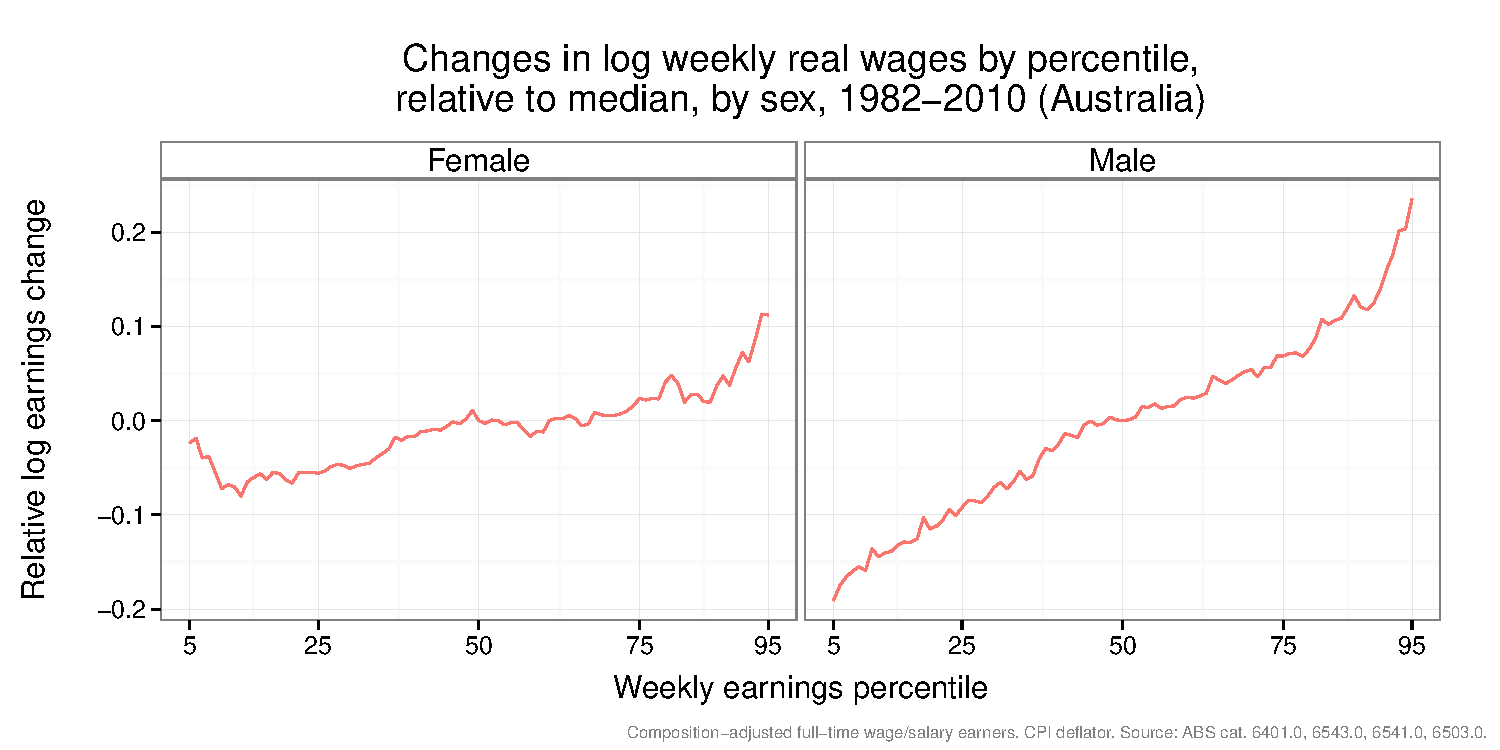
\includegraphics[width=\textwidth]{../figure/quantile_mf.pdf}
  \caption{Change in weekly wage by percentile, 1981-2010, Males and Females. Full-time workers whose main sources of income are wages and salaries are shown. Notice that real wage growth has been non-monotone for males in lower percentiles. Source: Survey of Income and Housing.}
  \label{fig:banana}
\end{figure}

\subsection{Does SBTC fit the Australian data?}

If SBTC explained the widening of the income distribution, we would expect to observe the premium accruing to `skilled' labor increasing with time. Figure~\ref{fig:banana} shows the composition-adjusted changes in log real wage by percentile, for males and females, between 1981-82 and 2009-10. If the 1981-82 income percentile can be considered a proxy for skill, then it is apparent that, over this period, wages more grew for high-skill individuals much faster than for low-skill individuals. It would therefore be expected that the premium accruing to higher educational attainment would show a similar trend.

In the United States, at least, the wage premium earned by tertiary-educated labor fell in the 1970s, but has risen each decade since then \citep{Acemoglu2011}. \citet{Katz1992} employs a similar empirical model which explains the rise of the skill premium in the United States in the post-war era. In Australia, however, a corresponding growth in the premium for tertiary qualifications has not been observed. Table~\ref{tbl:wagepremium} shows the log skill premium for Australia and the United States between 1982 and 2008. Rather than any fundamental differences in the nature of the demand for skills, \citet{Coelli2009} attributes this difference in Australian workers to differences in the nature of Australian educational qualifications. In Australia, University degrees are available to a wider range of candidates and for a wider range of disciplines than those who would traditionally have undertaken university studies in the United States. As a result, tertiary educational attainment may be a poor proxy for `skilled' work in Australia.
\begin{table}
  \centering
  \begin{tabular}{lcc}
  \hline
           & \multicolumn{2}{c}{\bf Log Skill Premium} \\
\hline
{\bf Year} &	{\bf United States} & {\bf Australia} \\
{\bf 1982} &	0.42 &	0.42 \\
{\bf 1995} &	0.59 &	0.36 \\
{\bf 2003} &	0.64 &	0.37 \\
{\bf 2008} &	0.68 &	0.34 \\ \hline
\end{tabular}
  \caption{University/non-university log wage premium, Australia and the United States. The figures show the difference between the mean log weekly income for workers who have attained a bachelor degree or higher, and the mean weekly income of other workers. Only full-time workers whose main sources of income are wages and salaries are included, and survey data have been composition adjusted for sex, age group, (and for the United States, race). Source: for Australia, ABS Survey of Income and Housing, and for the United States, \citet{Acemoglu2011}.}
  \label{tbl:wagepremium}
\end{table}

The SBTC model also claims that, even if technology exhibits skill bias, wages for all skill groups should increase monotonically. Figure~\ref{fig:changetime} plots the cumulative change over time for three wage percentiles, the 5th, 95th, and the median. Over the period 1981-82 to 2009-10, although wages at the top percentiles increased steadily, the same is not true for the lower percentiles. Indeed, for all of the 1990s and much of the 2000s, cumulative real income growth from 1981-82 was negative for many workers.
\begin{figure}
  \centering
  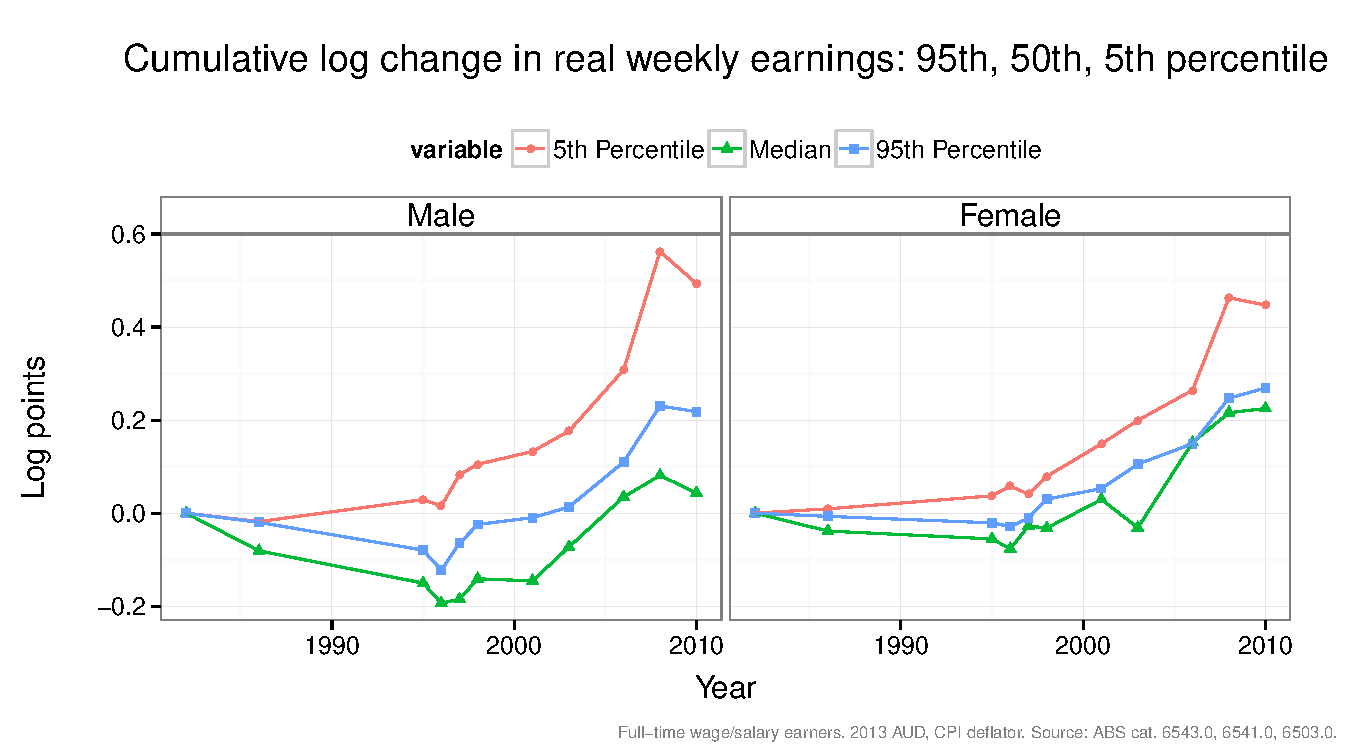
\includegraphics[width=\textwidth]{../figure/wage_change_time.pdf}
  \caption{Cumulative log change in real weekly earnings, 5th, 50th and 95th percentiles, 1982-2010. Full-time workers whose main sources of income are wages and salaries are shown. Notice that real wage growth has been non-monotone for males in lower percentiles. Source: Survey of Income and Housing.}
  \label{fig:changetime}
\end{figure}

That the income distribution is widening, but the skill premium is {\em not} driving the change, suggests one of at least two interpretations. We have already discussed the fact that educational attainment may be a poor indicator of skill for the Australian labor market. A second, more nuanced explanation was given by \citet{Levy2003}. Technological change may not be complementary to all types of labor; it may replace many types of labor entirely.





%%% Local Variables: 
%%% mode: latex
%%% TeX-master: "thesis"
%%% End: 
